\section{What Did Not Work}
\label{sec:failed}

The leak-free gap motivated many attempts. We report them because a reader should know which common ideas have been tried on these data and how they fared.

\subsection{G27: One Recipe for All Protocols}
Diagnostics said three things: RF-DETR's box extent is at the annotator ceiling, its candidate recall is high, and rare-class scoring is where it loses, with post hoc rescoring closed. G27 therefore changed what the model learns from, with three additions on one pre-registered path:
\begin{itemize}
\item \textbf{CP:} copy-paste~\cite{copypaste} of real boxes from the same training set into classes below the median count (Fig.~\ref{fig:copypaste}).
\item \textbf{D1:} in-domain self-supervised adaptation of RF-DETR's DINOv2 encoder by masked feature distillation~\cite{data2vec}, on a leak-checked pool of 22{,}318 images.
\item \textbf{D2:} a multi-dataset supervised stage 1 on the same pool, with partitioned class slots~\cite{multidataset}.
\end{itemize}
Phase A-1 selected the recipe R on validation (seed 0): the best mean among arms that beat A0 on both datasets. Phase A-2 is the primary test claim on seeds 0 and 1: R $-$ A0 $>0$ on each dataset, with pooled $P(>0)\geq0.95$.

\begin{figure}[!t]
\centering
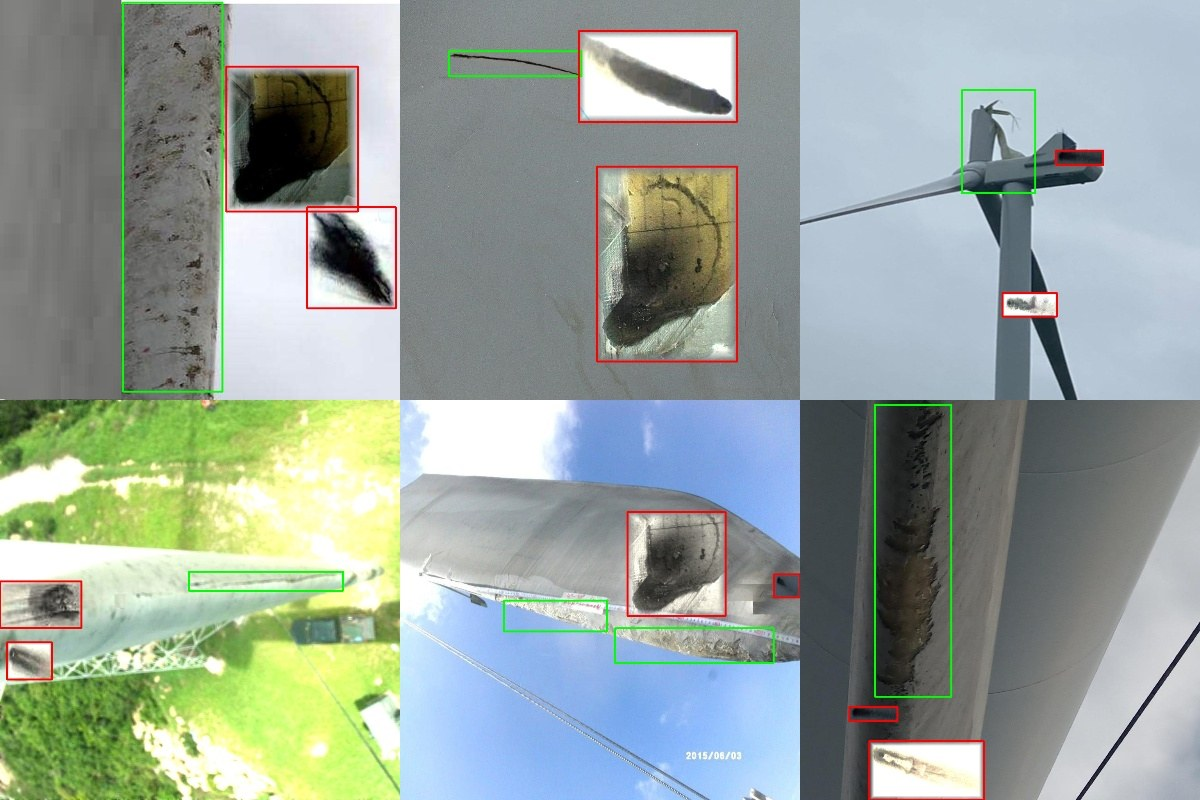
\includegraphics[width=0.9\linewidth]{fig25_cp_check}
\caption{Visual check of copy-paste before training. Some pastes land off the blade where SAM's~\cite{sam2} largest mask includes sky, and box-level pastes carry their source background. These were kept, since A1 $-$ A0 measures the recipe as it ran.}
\label{fig:copypaste}
\end{figure}

\begin{table}[!t]
\centering
\caption{G27 A-2, R = A1 (copy-paste): R $-$ A0, test \mcoco, mean of seeds 0 and 1. The primary claim fails.}
\label{tab:g27}
\footnotesize
\begin{tabular}{@{}l r l r@{}}
\toprule
& R $-$ A0 & 95\% CI & $P(>0)$ \\
\midrule
WTBD-group & $-0.99$ & \ci{-8.6}{+1.2} & 0.193 \\
WTBlade-group & $+0.35$ & \ci{-0.5}{+1.6} & 0.812 \\
mean over datasets & $-0.32$ & \ci{-4.1}{+0.9} & 0.290 \\
\bottomrule
\end{tabular}
\end{table}

\begin{table}[!t]
\centering
\caption{All G27 arms, \mcoco. Validation decided R; test was not used for selection. \hlnote{} (validation, the selection criterion)}
\label{tab:g27val}
\footnotesize
\setlength{\tabcolsep}{2.5pt}
\begin{tabular}{@{}l r l r l@{}}
\toprule
& \multicolumn{2}{c}{WTBD-group} & \multicolumn{2}{c}{WTBlade-group} \\
\cmidrule(lr){2-3}\cmidrule(l){4-5}
Arm & val s0 & test s0/s1 & val s0 & test s0/s1 \\
\midrule
A0 plain & \second{40.11} & 33.2/32.2 & 15.68 & 16.2/16.9 \\
A1 + CP & \best{40.15} & 30.7/32.7 & \second{17.10} & 17.3/16.5 \\
A2 + CP + D1 & 34.2 & 27.4/-- & 15.6 & 16.1/-- \\
A3 + CP + D2 & 33.4 & 33.2/-- & \best{17.7} & 16.6/-- \\
\bottomrule
\end{tabular}
\end{table}

\begin{figure}[!t]
\centering
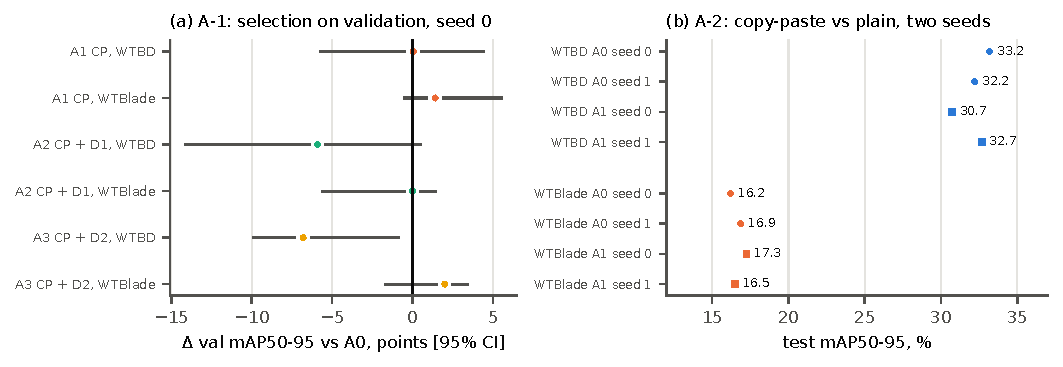
\includegraphics[width=\linewidth]{fig16_g27}
\caption{G27. (a) A-1, validation deltas against A0, seed 0. (b) A-2, test by seed: the seed swing is as large as the effect.}
\label{fig:g27}
\end{figure}

R $=$ A1 was chosen by $+0.04$ points on WTBD-group validation, smaller than A0's own seed-to-seed difference on validation (Tables~\ref{tab:g27}, \ref{tab:g27val}; Fig.~\ref{fig:g27}). Without the residual pixel-twin images, R $-$ A0 is $-1.01$ on WTBD-group and $+0.40$ on WTBlade-group, so the conclusion is unchanged. D1 and D2 were rejected on A-1 ($-5.9$ and $-6.8$ points against A1 on WTBD validation). A post hoc check found that D1 halved the effective rank of the encoder's last stage (257 to 135), a partial dimensional collapse. This finding motivated keeping the prior frozen in RF-DETR-FP. A seed swing of up to 2 points on these test sets (A1 on WTBD: 30.7 and 32.7) sets the smallest effect that can be claimed.

\subsection{Semi-Supervised Learning}
Label budgets suggested semi-supervision, and it took three rounds to rule out (Table~\ref{tab:ssl}). The idea was distinctive: drone inspection produces overlapping real views of the same surface, which our audit registers with verified transforms (about 4{,}000 WTBD and 70{,}000 WTBlade pairs). A teacher's detections on one view can be mapped into another and used as pseudo-labels~\cite{meanteacher,unbiasedteacher,softteacher}. Seed noise alone is $\pm2.6$ \mfifty at 25\%, as wide as every effect we measured. The class-balanced variant is significantly worse, partly through a confirmation-bias runaway: one seed produced up to about 2{,}300 pseudo-boxes per epoch from 24 images. Measured against hidden labels, even a good teacher's pseudo-labels are 66\% correct at threshold 0.5 and 40\% at 0.25.

\begin{table}[!t]
\centering
\caption{Teacher--student rounds at 25\% of WTBD-group~\cite{meanteacher}. Top: one seed per arm, COCO-style evaluator. Bottom: three seeds per arm. \hlnote{} (within each block)}
\label{tab:ssl}
\footnotesize
\setlength{\tabcolsep}{2.4pt}
\begin{tabularx}{\linewidth}{@{}X l l r@{}}
\toprule
Arm & Test 50 / 50:95 & Val best & Pseudo \\
\midrule
supervised & \best{23.2} / \best{8.2} & 44.4 / \second{22.6} & -- \\
synthetic views, unlabelled pool & \second{22.4} / 7.8 & \second{44.8} / 22.0 & 2{,}748 \\
real views, unlabelled pool & 19.2 / 7.7 & 38.2 / 18.4 & 961 \\
in-domain (rest of train, labels hidden) & 20.9 / \second{8.0} & \best{45.7} / \best{22.7} & 1{,}294 \\
\midrule
supervised, 3 seeds & \best{21.3}$\pm$2.6 / \best{7.9}$\pm$1.0 & & -- \\
class-balanced in-domain, 3 seeds & 16.3$\pm$2.0 / 6.6$\pm$0.6 & & up to 28{,}742 \\
\bottomrule
\end{tabularx}
\end{table}

\subsection{The Ledger}
Table~\ref{tab:ledger} lists the method hypotheses we ran or formally gated, with their results, and Fig.~\ref{fig:failed} plots those with a test effect in points. Some effects are real but narrow, such as copy-paste on rare classes in a low-label setting. Few survive a second dataset or a replication. Several directions were also discarded before any run, after literature or ceiling checks showed little room. These include box-extent refinement (RF-DETR is at the annotator ceiling, Table~\ref{tab:ceiling}), a crop re-classifier, policy-gradient training on mAP~\cite{raopg} as such, point-supervised boxes~\cite{pointdetr} and prototype rescoring~\cite{attentionrpn}, which is prior art in few-shot detection.

\begin{figure}[!t]
\centering
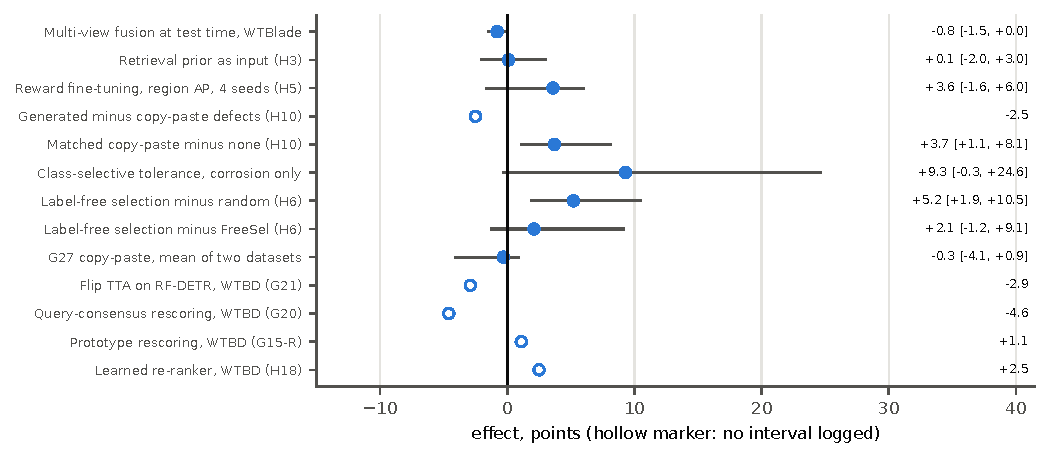
\includegraphics[width=\linewidth]{fig22_failed_tests}
\caption{Effects of method tests on leak-free test sets, in \mcoco points unless the ledger says otherwise; WTBD-group unless labelled. Hollow markers: no interval was logged in that form.}
\label{fig:failed}
\end{figure}

\begin{table*}[!t]
\centering
\caption{Ledger of method tests and diagnostics, in order of registration (H: hypothesis; G: gate). WTBD-group, test \mcoco points unless noted. Pre-registered from late October; earlier rounds were decided in advance but not formally committed.}
\label{tab:ledger}
\footnotesize
\begin{tabularx}{\textwidth}{@{}l X X l@{}}
\toprule
Test & Idea & Result & Verdict \\
\midrule
Phases 22--24 & Teacher--student with synthetic or real views, in-domain, class-balanced; 3 seeds & balanced in-domain 6.6 vs.\ supervised 7.9; \mfifty $-4.2$ \ci{-12.1}{-0.3}; runaway on one seed & fails \\
Phase 24 & SAM 2.1 box refinement~\cite{sam2} & $+0.3$ to $+0.5$ at 25\%, $-0.2$ at 100\% & fails \\
Phases 18, 26 & Split-tolerant training; class-selective version, 2 seeds & blanket not an improvement; corrosion $+9.3$ \ci{-0.3}{+24.6}, mean $-0.4$ & targeted only \\
H1 & Multi-view fusion at test time & untestable on WTBD (26 images with a second view); WTBlade-group $-0.8$ \ci{-1.5}{0.0} & fails \\
H2 & Normal-blade anomaly prior from DINOv3 patches & most anomalous patches not on defects; box recall below chance & fails \\
H3 & Retrieval prior (nearest labelled patches) as a detector input & $+0.1$ \ci{-2.0}{+3.0} & fails \\
H4 & Test-time adaptation across real views & gate failed: real views do not make better detections & not run \\
H5 & Reward fine-tuning with a granularity-invariant reward; 4 seeds + WTBlade & region AP $+3.6$ \ci{-1.6}{+6.0}, $P$ 0.896; WTBlade $-0.6$ & fails on replication \\
H6 & Label-free scene selection by patch coverage & $+5.2$ \ci{+1.9}{+10.5} over random; $+2.1$ \ci{-1.2}{+9.1} over FreeSel & no gain over prior art \\
H7 & Label-free property predicting subset quality & no property survives correction & fails \\
H8, H9 & Feature upsampling; high-frequency cues & $-5.9$; $-0.1$ & fail \\
H10 & Generated rare-class defects vs.\ matched copy-paste & synth $-$ paste $-2.5$; paste $-$ none $+3.7$ \ci{+1.1}{+8.1} & generation fails \\
H12 & DINOv3 reduces subset luck & it does not; draw quality carries over ($\rho$ 0.71) & fails \\
G15, G15-R & Prototype rescoring with DINOv3 box embeddings & WTBD $+1.1$; WTBlade $-0.7$ & fails bar; prior art \\
G16, G16-R & Instance-level proximity law; does it explain subset luck? & holds per instance; does not explain luck; on RF-DETR it governs confidence, not detection & partial \\
G17 & Clicks as pseudo-boxes (bar 60\% at IoU $\geq$0.5) & 42.0\% & fails \\
H18, -R, -W & Learned coverage-aware re-ranker on RF-DETR & WTBD $+2.5$, replicated on new models; WTBlade $+0.2$ & WTBD only \\
H19-W & Rescoring at the low-count boundary, WTBlade 8\% & $-0.2$ \ci{-1.3}{+0.7}, $P$ 0.286 & fails \\
G20 & Query-consensus rescoring & $-4.6$ WTBD; $-2.1$ WTBlade & fails \\
G21 & Flip agreement; plain flip TTA on RF-DETR & $-2.9$ WTBD; $-0.6$ WTBlade & fails; TTA hurts \\
G22, -O & Fine-tuning moves proximity from recall to ranking & confirmed on WTBD with a frozen-encoder control; not on WTBlade & does not replicate \\
H20 & Subset luck as annotation-convention match & no relation & fails \\
G24 & Input resolution 768 vs.\ 576 & WTBD $+1.0$ ($P$ 0.958); WTBlade $-0.1$ & dataset-specific \\
V1 & RF-DETR replaces the frozen-feature detector at 25\% & $+7.3$ \ci{+2.3}{+11.9}; $+8.3$ \ci{+4.5}{+15.0} & passes \\
G25, G26 & Official-protocol benchmark; tuned recipe & Tables~\ref{tab:official}, \ref{tab:tuning} & reported \\
G27 & CP, D1, D2 recipe & A-2 $-0.32$, $P$ 0.290 & fails \\
G28 & Leave-one-dataset-out & dead on both targets & fails \\
G29 & RF-DETR-FP, frozen DINOv3 prior & P $+1.45$, $P$ 0.958 (val $+0.20$); S $+1.38$, $P$ 0.856 & P passes narrowly; S fails \\
\bottomrule
\end{tabularx}
\end{table*}
